
\section{Calculations \& Graphs}

\vspace{-0.5cm}
\singlespacing

%------- Force --------%

\subsection{Normal Force} 

{\centering
\begin{equation}
	F_N = F_w = mg
	\label{eq:nForce}
\end{equation}
\begin{align*}
	\boldsymbol{F_N} &: \text{Normal Force} \\
	\boldsymbol{F_w} &: \text{Weight} \\
	\boldsymbol{m} &: \text{mass of object} \\
	\boldsymbol{g} &: \text{acceleration due to gravity}
\end{align*}}

\subsubsection{Sample Calculation \\ {\normalfont \small\textit{Normal force of box with 1 kg of mass inside}}}

{\centering
\begin{align*}
	F_N &= F_w = mg \\
			&= F_w = (2.293\,\text{kg})(9.8\,\text{m/s$^2$}) \\
			&= F_w = 22.47\,\text{N} \\
	F_N &= \boxed{22.47\,\text{N}}
\end{align*}}

\subsection{Kinetic Friction Force}

{\centering
\begin{equation}
	F_k =\mu_k F_N 
	\label{eq:kFriction}
\end{equation}
\begin{align*}
	\boldsymbol{F_k} &: \text{Force of kinetic friction} \\
	\boldsymbol{\mu_k} &: \text{Coefficient of kinetic friction} \\
	\boldsymbol{F_N} &: \text{Normal force} \\
	\boldsymbol{g} &: \text{acceleration due to gravity}
\end{align*}}

\subsubsection{Sample Calculation \\ {\normalfont \small\textit{Determining coefficient of friction using wooden box acceleration from Part 3 trial 1}}}

{\centering
\begin{align*}
	F_k &= \mu_k F_N \\
	2.498\,\text{N} &= (\mu_k)(12.6714\,\text{N}) \\
	\mu_k &= \boxed{0.1971}
\end{align*}}


\newpage

%------- AVERAGE VALUE --------%
\subsection{Average Value Formula} 

\begin{align*}
	\overline{a} = \frac{\text{sum of values}}{\text{total \# of values}} 
\end{align*}

\subsubsection{Sample Calculation \\ {\normalfont \small\textit{average static friction with 1000 g in wooden box}}}


\begin{align*}
	\overline{a}&=\frac{\text{sum of values}}{\text{total \# of values}} \\ \\
							&= \frac{2.847+3.332+3.362}{3} \\ \\
	\overline{a}&= \boxed{3.180\,\text{N}}
\end{align*}
%------- AVERAGE VALUE --------%

%------- STANDARD DEVIATION --------%
\subsection{Standard Deviation Formula}

\begin{align*}
		\sigma &= \sqrt{\frac{\Sigma(x_i -\overline{a})^2}{N}} \\
		 &= \sqrt{\frac{SS}{N}} \\ \\
		\textbf{N} &:\, \text{Total number of values} \\
		\overline{\textbf{a}} &:\, \text{Average value} \\
		\textbf{x\textsubscript{i}} &:\, \text{Each value from the data set} \\
		\textbf{SS} &:\, \text{Sum of squares} 
\end{align*}

\subsubsection{Sample Calculation \\ {\normalfont \small\textit{std of static friction in Part 2 with 1000 g in wooden box }}}

\begin{align*}
	\sigma &= \sqrt{\frac{(2.847-\overline{a})^2 + ... + (3.362-\overline{a})^2}{3}} \\
		 &= \sqrt{\frac{0.16711667}{3}} \\
		 &= \boxed{0.236\, \text{N}}
\end{align*}
%------- STANDARD DEVIATION --------%


%----TABLES-----%


\subsection{Part 1: Starting Friction}

\begin{table}[H]
\centering
\resizebox{4cm}{!}{%
\begin{tabular}{@{}c@{}}
\toprule
\textbf{Mass of block (kg)} \\ \midrule
1.293                       \\ \bottomrule
\end{tabular}%
}
\caption{Part 1: Starting Friction}
\label{tab:massBox}
\end{table}

\subsection{Part 2: Peak Static Friction and Kinetic Friction}

\begin{table}[H]
\captionsetup{font=large}
\caption{Part 2: Peak Static Friction}
\centering
\begin{threeparttable}
\resizebox{\columnwidth}{!}{%
\begin{tabular}{cccccc} 
\toprule
\multicolumn{6}{c}{\textbf{Peak Static}}                                                                                   \\ 
\toprule
\textbf{Total mass (g)}             & \textbf{1000} & \textbf{800}   & \textbf{600}   & \textbf{400}   & \textbf{200}     \\ 
\toprule
\textbf{Normal Force (N)\tnote{!}}           & 22.47         & 20.51          & 18.55          & 16.59          & 14.63            \\
\textbf{Trial 1 (N)}                 & 2.847         & 2.392          & 1.877          & 1.483          & 0.9376           \\
\textbf{Trial 2 (N)}                 & 3.332         & 2.544          & 1.726          & 1.332          & 0.9376           \\
\textbf{Trial 3 (N)}                 & 3.362         & 3.12           & 1.786          & 1.301          & 0.9073           \\
\textbf{Standard Deviation (N)}      & 0.236         & 0.3135         & 0.06207        & 0.0795         & 0.01428          \\ 
\toprule
\textbf{Average static friction (N)} & \textbf{3.18} & \textbf{2.685} & \textbf{1.796} & \textbf{1.372} & \textbf{0.9275}  \\
\bottomrule
\end{tabular}%
}
\begin{tablenotes}\normalsize
	\item[!] Calculated with mass of block added to total mass inside block. 
\end{tablenotes}
\end{threeparttable}
\label{tab:part2s}
\end{table}

\begin{table}[H]
\captionsetup{font=large}
\caption{Part 2: Peak Kinetic Friction}
\centering
\begin{threeparttable}
\resizebox{\columnwidth}{!}{%
\begin{tabular}{cccccc} 
\toprule
\multicolumn{6}{c}{\textbf{Peak Kinetic}}                                                                                    \\ 
\toprule
\textbf{Total mass (g)}              & \textbf{1000}  & \textbf{800}   & \textbf{600}   & \textbf{400}   & \textbf{200}     \\ 
\toprule
\textbf{Normal Force (N)\tnote{!}}            & 22.47          & 20.51          & 18.55          & 16.59          & 14.63            \\
\textbf{Trial 1 (N)}                  & 2.405          & 2.005          & 1.561          & 1.115          & 0.7748           \\
\textbf{Trial 2 (N)}                  & 2.35           & 1.887          & 1.572          & 1.13           & 0.7749           \\
\textbf{Trial 3 (N)}                  & 2.407          & 1.97           & 1.561          & 1.131          & 0.7687           \\
\textbf{Standard Deviation (N)}       & 0.02641        & 0.04948        & 0.005185       & 0.007318       & 0.002899         \\ 
\toprule
\textbf{Average kinetic friction (N)} & \textbf{2.387} & \textbf{1.954} & \textbf{1.564} & \textbf{1.125} & \textbf{0.7728}  \\
\bottomrule
\end{tabular}%
}
\begin{tablenotes}\normalsize
	\item[!] Calculated with mass of block added to total mass inside block. 
\end{tablenotes}
\end{threeparttable}
\label{tab:part2k}
\end{table}

%----GRAPHS-----%

\subsubsection{Graphs}
\begin{figure}[H]
	\begin{center}
		\captionsetup{font=large}
		\caption{Static Friction vs. Normal Force}\label{fig:SFvNF}
		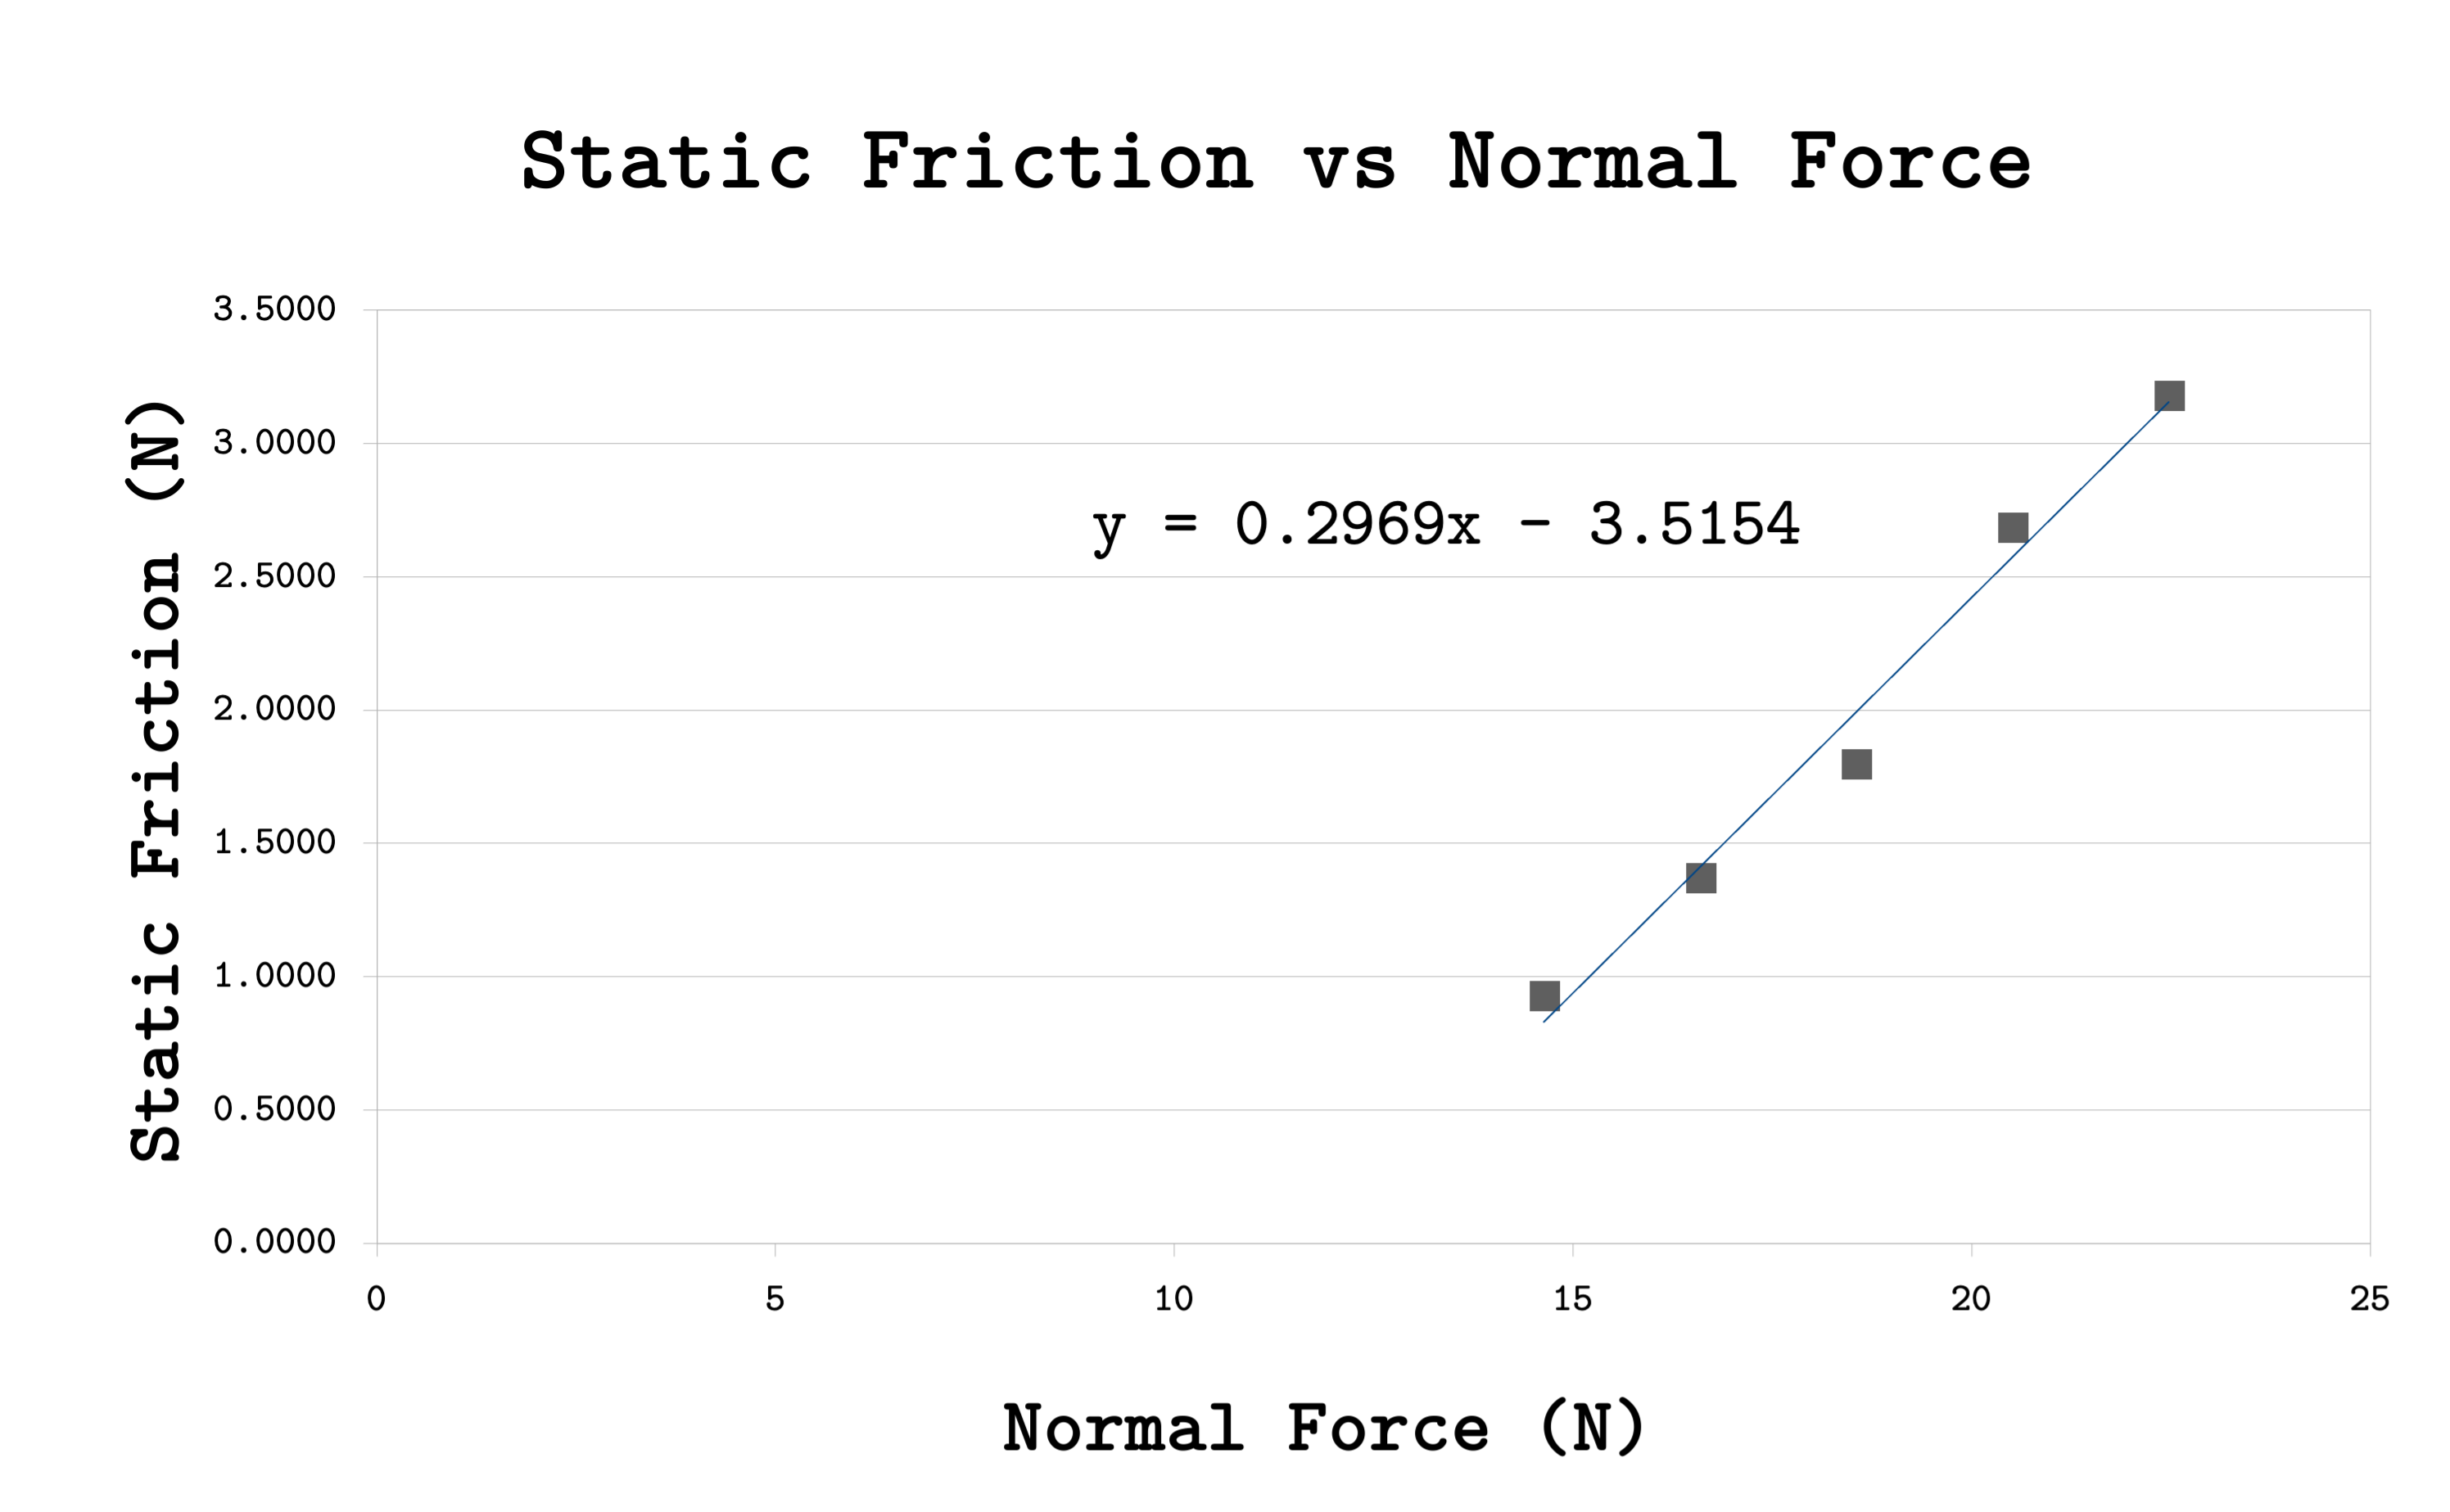
\includegraphics[width=0.90\columnwidth]{images/GraphSFvNF}
	\end{center}
\end{figure}


\begin{figure}[H]
	\begin{center}
		\captionsetup{font=large}
		\caption{Kinetic Friction vs. Normal Force}\label{fig:KFvNF}
		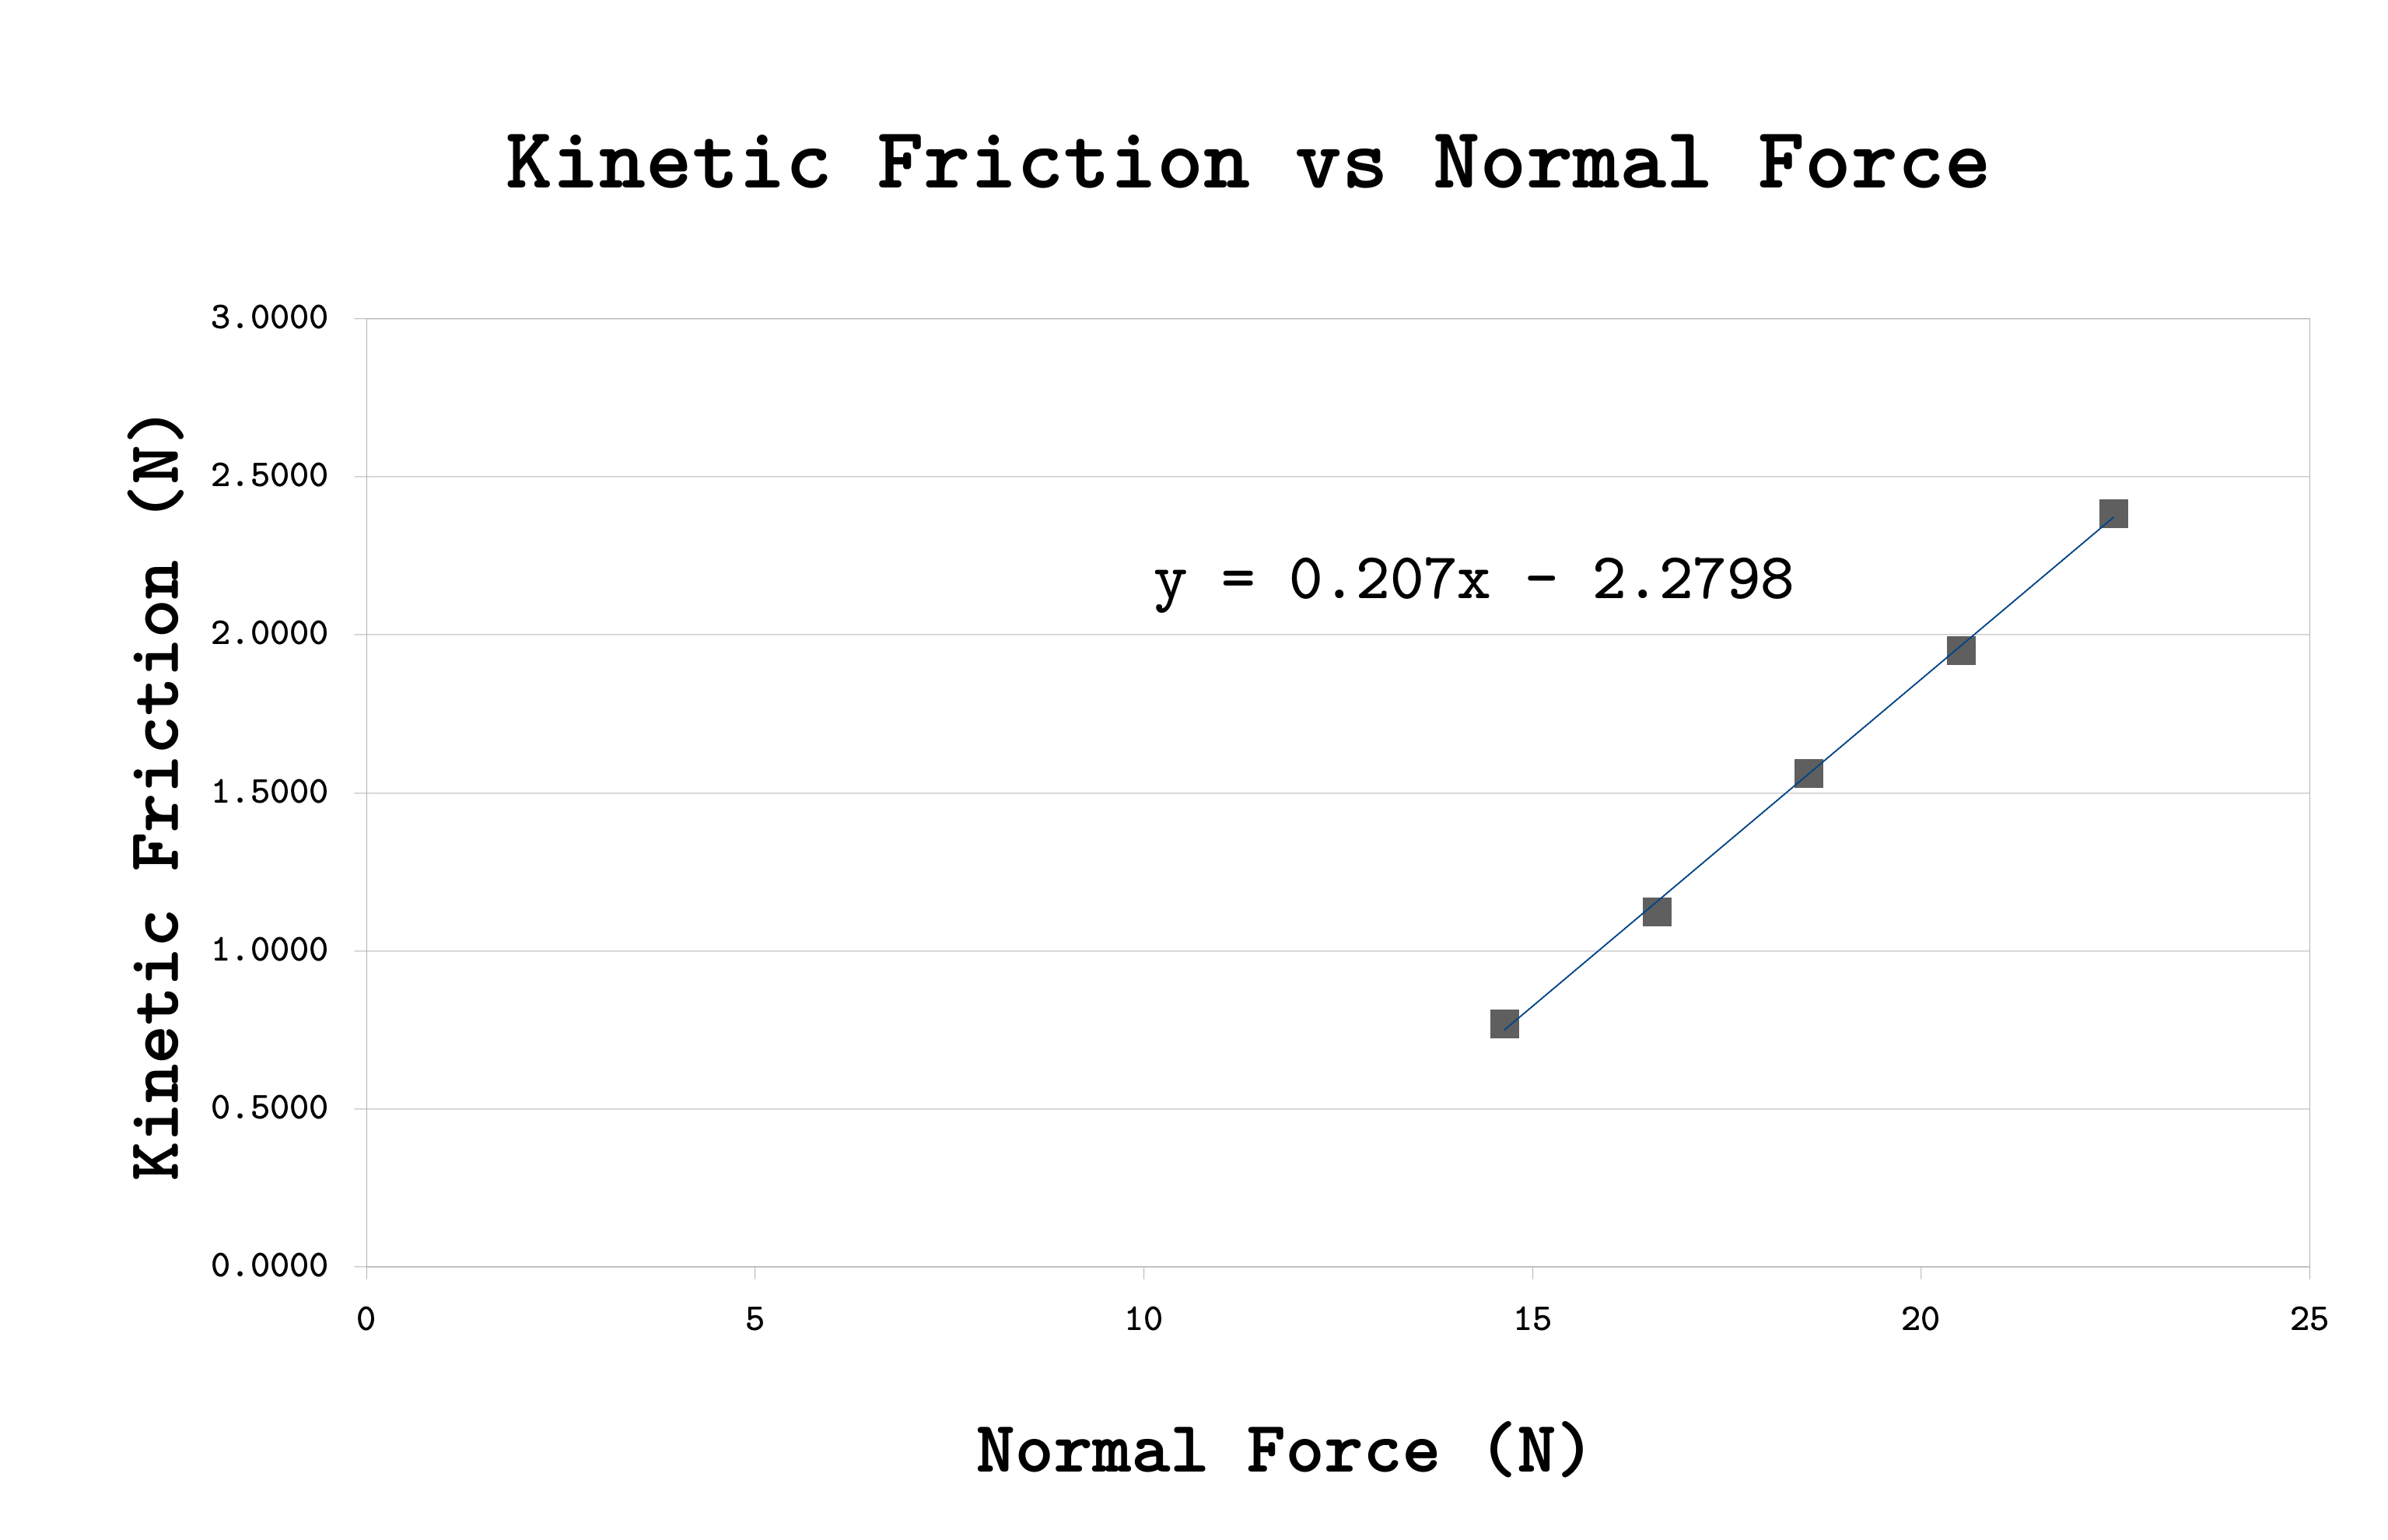
\includegraphics[width=0.90\columnwidth]{images/GraphKFvNF}
	\end{center}
\end{figure}

%----GRAPHS-----%

\subsection{Part 3: Kinetic Friction}

\begin{table}[H]
	\caption{Part 3: No additional mass}
\centering
\begin{tabular}{cccc} 
\toprule
\textbf{Trial} & \textbf{Acceleration (m/s\textsuperscript{2})} & \textbf{Kinetic Friction Force (N)} & $\boldsymbol{\mu_k}$  \\ 
\toprule
\textbf{1}     & 1.932                                          & 2.4980                              & 0.1971            \\
\textbf{2}     & 2.061                                          & 2.6640                              & 0.2103            \\
\textbf{3}     & 2.103                                          & 2.7190                              & 0.2146            \\
\textbf{4}     & 1.816                                          & 2.3480                              & 0.1853            \\
\textbf{5}     & 1.723                                          & 2.2270                              & 0.1758            \\ 
\toprule
							 &                                                & \textbf{Average $\boldsymbol{\mu_k}$}             & \textbf{0.1966}   \\
\toprule
\end{tabular}
\label{tab:part3block}
\end{table}

 
\begin{table}[H]
	\caption{Part 3: Block with 500 g of additional mass}
\centering
\begin{tabular}{cccc} 
\toprule
\textbf{Trial} & \textbf{Acceleration (m/s\textsuperscript{2})} & \textbf{Kinetic Friction Force (N)} & $\boldsymbol{\mu_k}$  \\ 
\toprule
\textbf{1}     & 2.092                                          & 2.7040                              & 0.2054            \\
\textbf{2}     & 1.828                                          & 2.3630                              & 0.1794            \\
\textbf{3}     & 2.044                                          & 2.6420                              & 0.2007            \\
\textbf{4}     & 2.03                                          & 2.6240                              & 0.1993            \\
\textbf{5}     & 2.095                                          & 2.7080                              & 0.2057            \\ 
\toprule
							 &                                                & \textbf{Average $\boldsymbol{\mu_k}$}             & \textbf{0.1981}   \\
\toprule
\end{tabular}
\label{tab:part3500g}
\end{table}
%----TABLES-----%


\newpage

